
\section{Sobre HASDE}

\subsection{¿Qué es HASDE?}

HASDE es una \textbf{H}erramienta abierta para \textbf{A}prendizaje interactivo del método de \textbf{S}lope \textbf{DE}flection. %
%
La herramienta permite que la persona que se encuentra aprendiendo la metodología de aplicación del Método de Slope Deflection para analizar pórticos, pueda verificar cada paso realizado e identificar posibles errores de forma autónoma.


HASDE está desarrollada utilizando GNU-Octave 5.1.0, utilizando las funciones de interfaz gráfica disponibles a partir de esta versión. %
%
La versión actual del código está disponible en el repositorio abierto: \href{https://github.com/grupomises/HASDE}{https://github.com/grupomises/HASDE}. 

\subsection{Apoyos}
El código fue desarrollado con el apoyo de la Comisión Sectorial de Enseñanza en el marco de la ejecución del proyecto de innovaciones educativas titulado: 
``Rediseño de prácticas de enseñanza y evaluación en Resistencia de Materiales''\footnote{ver resumen público de proyecto en	\href{https://www.cse.udelar.edu.uy/blog/proyecto-financiado/rediseno-de-practicas-de-ensenanza-y-evaluacion-en-resistencia-de-materiales/}{https://www.cse.udelar.edu.uy/blog/proyecto-financiado/rediseno-de-practicas-de-ensenanza-y-evaluacion-en-resistencia-de-materiales/}}.

\subsection{Licencia}

Este código es publicado bajo licencia GNU-GPL 3.0. Está distribuido con el objetivo de que sea útil pero sin ningún tipo de garantía. Ver el archivo LICENSE por detalles.


\section{Ejemplo demostrativo}

Para mostrar el funcionamiento del código se desarrolla un ejemplo demostrando el desarrollo a ser realizado por la persona que utilice la herramienta. Se comienza con la resolución analítica del ejemplo para luego pasar al ingreso de los cálculos en HASDE para su verificación.

\subsection{Planteo de problema}

Sea la estructura mostrada en la \autoref{fig:ejem} donde las barras tienen módulo de Young $E=210 \times 10^{6}$ kPa y sección transversal $0.05 \text{m} \times 0.05$ m, es decir que $EI=109.4 $ kNm$^2$. %
También se conoce que $P = 1350$ kN.



Se desea determinar desplazamientos y giros nodales. %

\begin{figure}[htb]
	\centering
	\def\svgwidth{0.5\textwidth}
	\input{figs/portic.pdf_tex}
	\caption{Pórtico de ejemplo.}
	\label{fig:ejem}
\end{figure}

\subsection{Resolución analítica}


\subsubsection{Determinación de incógnitas}
La estructura es desplazable y el desplazamiento horizontal de $2$ es una incógnita a determinar. %
%
Se utilizará como variable el desplazamiento horizontal del piso $2-3$, denotado como $\Delta$ considerado positivo hacia la izquierda. %
%
Las otras variables a determinar son los giros $\theta_2$ y $\theta_3$. %
Por lo tanto 
$$
\boxed{\text{Número de incógnitas: } 3},
$$
siendo:
$$
\boxed{
 \theta_2, \theta_3 \text{ y } \Delta}
$$
donde $\Delta$ es el desplazamiento horizontal.


Se utilizarán en todas las ecuaciones las condiciones de contorno: desplazamientos y giros nulos en $1$ y 2.


\subsubsection{Ecuaciones de solicitaciones por elemento}

Las ecuaciones de equilibro que se usarán para aplicar el método son: las de equilibrio de momentos en 2, equilibrio de momentos en 3 y equilibrio de fuerzas en el piso. Para esto se calculan a continuación algunas de las fuerzas y momentos nodales que serán necesarias.

\paragraph{Ecuaciones de momentos}


Usando la ecuación de momento en 1 en la barra 1-2 se tiene:
$$
M_{12} = \frac{2EI}{6} \left( \theta_2 - 3 \frac{ \Delta } {6} \right).
$$

sustituyendo $EI$ se tiene:

\begin{equation}
\boxed{
	M_{12}  = 36.47 \theta_2 - 18.2 \Delta}
\end{equation}

Usando la ecuación de momento en 2 en la barra 2-1 se tiene:
$$
	M_{21} = \frac{2EI}{6} \left( 2\theta_2 - 3 \frac{ \Delta } {6} \right).
$$

sustituyendo $EI$ se tiene%
\begin{equation}
\boxed{
M_{21}  = 72.9 \theta_2 - 18.2 \Delta}
\end{equation}
 
Usando la ecuación de momento en 2 en la barra 2-3 se tiene:
$$
	M_{23} = \frac{2EI}{9} \left(2\theta_2 +\theta_3 \right) + \frac{ P \cdot 3 \cdot 6^2}{9^2}
$$

sustituyendo $EI$:
%
\begin{equation}
\boxed{
M_{23} = 48.6 \theta_2 + 24.3 \theta_3  + 1800
}
\end{equation}

Para la barra 2-3, utilizando la ecuación de momento en 3 se tiene:
$$
M_{32} = \frac{2EI}{9} \left(2\theta_3 +\theta_2 \right) - \frac{P \cdot 3^2 \cdot 6}{9^2}
$$
sustituyendo $EI$ se tiene:

\begin{equation}
\boxed{
M_{32} = 48.6 \theta_3 + 24.3 \theta_2 - 900
}
\end{equation}

Planteando la ecuación de momento en 3 para la barra 3-4 se tiene:

$$
M_{34} = \frac{2EI}{9} \left(2\theta_3 - \frac{3}{9} \Delta \right)
$$

sustituyendo $EI$ se tiene:

\begin{equation}
\boxed{
	M_{34} = 48.6 \theta_3 - 8.1 \Delta
}
\end{equation}

Planteando la ecuación de momento en 4 para la barra 3-4 se tiene:

$$
M_{43} = \frac{2EI}{9} \left(\theta_3 - \frac{3}{9} \Delta \right)
$$

sustituyendo $EI$ se tiene:

\begin{equation}
\boxed{
	M_{34} = 24.31 \theta_3 - 8.1 \Delta
}
\end{equation}

\paragraph{Ecuaciones de fuerzas nodales}


Planteando la ecuación de cortante en 2 para la barra 2-1, se tiene:

$$
F_{21} = \frac{-(M_{21}+M_{12})}{6}
$$
sustituyendo $EI$ se tiene:

\begin{equation}
\boxed{
	F_{21} = -18.22 \theta_2 + 6.08 \Delta
}
\end{equation}

Planteando la ecuación de cortante en 3 para la barra 3-4, se tiene:

$$
F_{34} = \frac{-(M_{34}+M_{43})}{6}
$$
sustituyendo $EI$ se tiene:

\begin{equation}
\boxed{
	F_{34} = -8.10 \theta_3 + 1.80 \Delta
}
\end{equation}

\subsubsection{Matriz de rigidez}

Para determinar la matriz de rigidez, se deben imponer condiciones para resolver la estructura. En el ejemplo las condiciones a imponer son las siguientes:


\begin{eqnarray}
	\left\lbrace 
	\begin{array}{l}
	M_{21}+M_{23} = 0 \\
	M_{32}+M_{34} = 0 \\
	F_{21}+F_{34} = 0
	\end{array}
	\right.
\end{eqnarray}

Sumando las ecuaciones determinadas anteriormente, se tiene:

\begin{eqnarray}
	\left\lbrace 
	\begin{array}{llll}
	121.56 \theta_{2} &+ 24.31 \theta_{3} &-18.23 +1800 &= 0\\
	24.31 \theta_{2} &+ 48.62 \theta_{3} &-8.10 -900  &= 0\\
	-18.23 \theta_{2} &-8.10 \theta_{3} &+7.88 &= 0
	\end{array}
	\right.
\end{eqnarray}

Por lo tanto, la matriz de rigidez resulta:

\begin{eqnarray}
	K = \left[
	\begin{array}{lll}
	121.56 &24.31  &-18.23 \\
	24.31 &48.62  &-8.10 \\
	-18.23  &-8.10 &7.88	
	\end{array}
	\right]
\end{eqnarray}

\subsubsection{Vector de fuerzas externas}

El vector de fuerzas externas se construye a partir de los términos independientes de las condiciones que se imponen para resolver el problema. Por lo tanto, el vector de fuerzas externas resulta:

\begin{eqnarray}
F_{ext} = \left[
\begin{array}{c}
-1800 \\
900 \\
0
\end{array}
\right]
\end{eqnarray}

En este caso los valores de este vector están en unidades kN o kNm según corresponda.
%
%
%
%
%
%\subsubsection{Ecuaciones de equilibrio}
%
%
%Usando el equilibrio de momentos en B ($M_{BA}+M_{BC}=0$) y simplificando se tiene
%\begin{equation}
%	\boxed{
%		2EI \left( 2 \left( \frac{1}{6}+\frac{1}{9} \right) \theta_B + \frac{1}{9} \theta_C - \frac{3 }{6^2} \Delta_{BC} \right) = - \frac{4}{3} P.
%	}
%\end{equation}
%
%Esta consiste en la primer ecuación que relaciona las tres incógnitas a determinar.
%
%
%
%
%Usando el equilibrio de momentos en C y simplificando se tiene:
%\begin{equation}
%	\boxed{
%		2EI \left( \frac{1}{9} \theta_B + \frac{4}{9} \theta_C - \frac{3 }{9^2} \Delta_{BC} \right) = \frac{2}{3} P.
%	}
%\end{equation}
%
%Finalmente la ecuación de equilibrio de cortantes del piso es equivalente a la ecuación:
%\begin{equation}
%	\frac{M_{AB}+M_{BA}}{L_{AB}}
%	+ 
%	\frac{M_{CD}+M_{DC}}{L_{CD}} = 0
%\end{equation}
%
%Calculando la expresiones de los momentos $M_{CD}$ y $M_{AB}$, sustituyendo y simplificando se obtiene:
%\begin{equation}
%	\boxed{
%		2EI \left( -\frac{3}{6^2} \theta_B - \frac{3}{9^2} \theta_C + 6 \left( \frac{1}{6^3} +  \frac{1}{9^3} \right) \Delta_{BC} \right) = 0.
%	}
%\end{equation}
%
%El sistema de ecuaciones lineales a resolver es entonces
%\begin{equation}
%	\bfK   
%	\left[
%	\begin{matrix}
%		\theta_B\\
%		\theta_C\\
%		\Delta_{BC}
%	\end{matrix}
%	\right]
%	=
%	P
%	\left[
%	\begin{matrix}
%		-4/3\\
%		2/3\\
%		0
%	\end{matrix}
%	\right]
%\end{equation}
%donde $\bfK$ es la matriz del sistema dada por: 
%\begin{equation}
%	\bfK =
%	2EI \left[
%	\begin{matrix}
%		2 \left( \frac{1}{6}+ \frac{1}{9}\right) & \frac{1}{9} & -\frac{3}{6^2}\\
%		\frac{1}{9} & \frac{4}{9} & -\frac{3}{9^2}\\
%		-\frac{3}{6^2} & -\frac{3}{9^2} &  6\left( \frac{1}{6^3}  + \frac{1}{9^3}\right)
%	\end{matrix}
%	\right]
%\end{equation}
%
%Esta matriz es la llamada matriz de rigidez. Previo a la resolución del sistema es importante verificar que la misma es simétrica. %
%%
%Para resolver se pueden ejecutar los siguientes comandos en Octave:
%
%\begin{verbatim}
%K = 2* [ 2*(1/6+1/9)  1/9         -3/6^2 ; ...
%1/9         4/9         -3/9^2 ; ...
%-3/6^2     -3/9^2    6*(1/6^3+1/9^3) ] ;
%u = K \ [-4/3; 2/3; 0]
%\end{verbatim}
%
%
%Obteniendo la solución:
%\begin{equation}
%	\theta_B = \frac{ -1.90385 P }{EI}, \theta_C = \frac{ 0.93930
%		P }{EI} \text{ y } \Delta_{BC} = \frac{-3.43990 P }{EI}
%\end{equation}


\subsection{Verificación usando HASDE}

En esta sección se explica sintéticamente el uso de HASDE para verificar la resolución analítica.

\subsubsection{Convenciones de signo y sistemas de coordenadas}

Los desplazamientos nodales horizontales $\delta_x$ son considerados positivos hacia la izquierda. %
%
Los desplazamientos nodales verticales $\delta_y$ son considerados positivos hacia arriba. 

Los sistemas de coordenadas locales de las barras verticales son considerados con el eje $y$ local orientado hacia la izquierda.



\subsubsection{Interfaz gráfica}
Al ejecutar la función HASDE.m en Octave (v5.1.0) se abre una interfaz gráfica como la que se muestra en la Figura~\ref{fig:int}. En la figura se muestra el resultado obtenido en Windows.

\begin{figure}[htb]
	\begin{center}
		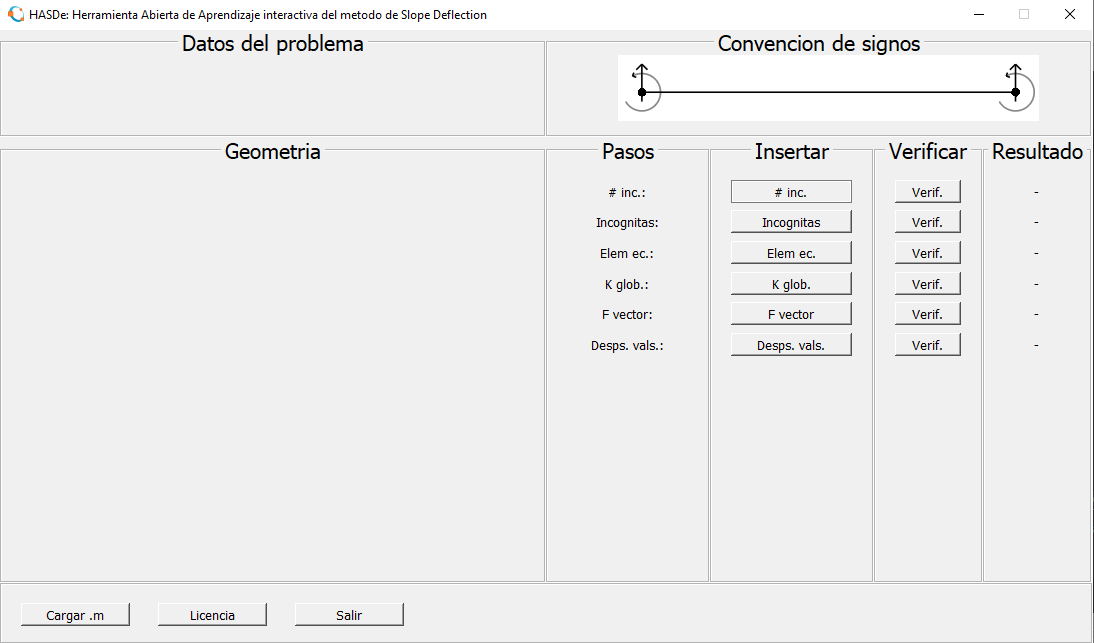
\includegraphics[width=\textwidth]{hasde.png}
	\end{center}
 \caption{Interfaz gráfica de inicio HASDE.}
 \label{fig:int}
\end{figure}
 
\paragraph{Cargar estructura}
Para resolver una estructura, se debe cargar un archivo de extensión \verb|.m| que contiene la información de la misma. Se puede acceder a dichos archivos mediante el botón \verb|Cargar .m| en el panel inferior.

\paragraph{Datos del problema}
En este panel se puede acceder a la información contenida dentro del archivo cargado con el fin de resolver la estructura.
En dichos botones se muestra el número de elemento, sus secciones y materiales, los nodos y sus coordenadas y los valores y la posición de las cargas que actúan sobre la estructura.

\paragraph{Geometría}
En este panel se muestra la estructura con la numeración de los nodos, las cargas que actúan y los apoyos. La convención utilizada para los apoyos es la siguiente:
\begin{itemize}
	\item Desplazamiento impedido: Se materializa mediante un triángulo en la dirección que restringe el desplazamiento. El momento flector en estos apoyos es nulo.
	\item Giro impedido: Se materializa mediante un cuadrado. En estos apoyos puede existir un momento flector.  
\end{itemize}

\paragraph{Convención de signos}
En este panel se muestra la convención de signos que se debe utilizar para resolver la estructura. Esta convención coincide con la utilizada en el método de Slope-Deflection.

\paragraph{Resolución}
Para la resolución de la estructura se deben seguir los pasos que se indican en en el panel \verb|Pasos|. Siguiendo estos pasos, se deben ingresar los correspondientes valores en el panel \verb|Insertar| y verificar los mismos mediante el botón \verb|Verif.|. Una vez realizada la secuencia anterior, en el panel \verb|Resultados| aparecerá el resultado de dicho paso.

\subsubsection{Pasos para la resolución}

\paragraph{\# Inc.}
En este paso, se deben ingresar la cantidad mínima de incógnitas para resolver la estructura. En el problema de ejemplo, dicho número es 3.

\paragraph{Incógnitas}
En este paso, se deben ingresar cuáles son dichas incógnitas, indicando el nodo e ingresando un 1 en el desplazamiento en el que ocurran.

En la Figura~\ref{fig:eje} se muestra la ventana de HASDE luego de haber ingresado correctamente el número de incógnitas y las propias incógnitas. En esta figura se muestra la salida en Arch Linux en una pantalla de resolución $3200 \times 1800$.
%
\begin{figure}[htb]
	\begin{center}
		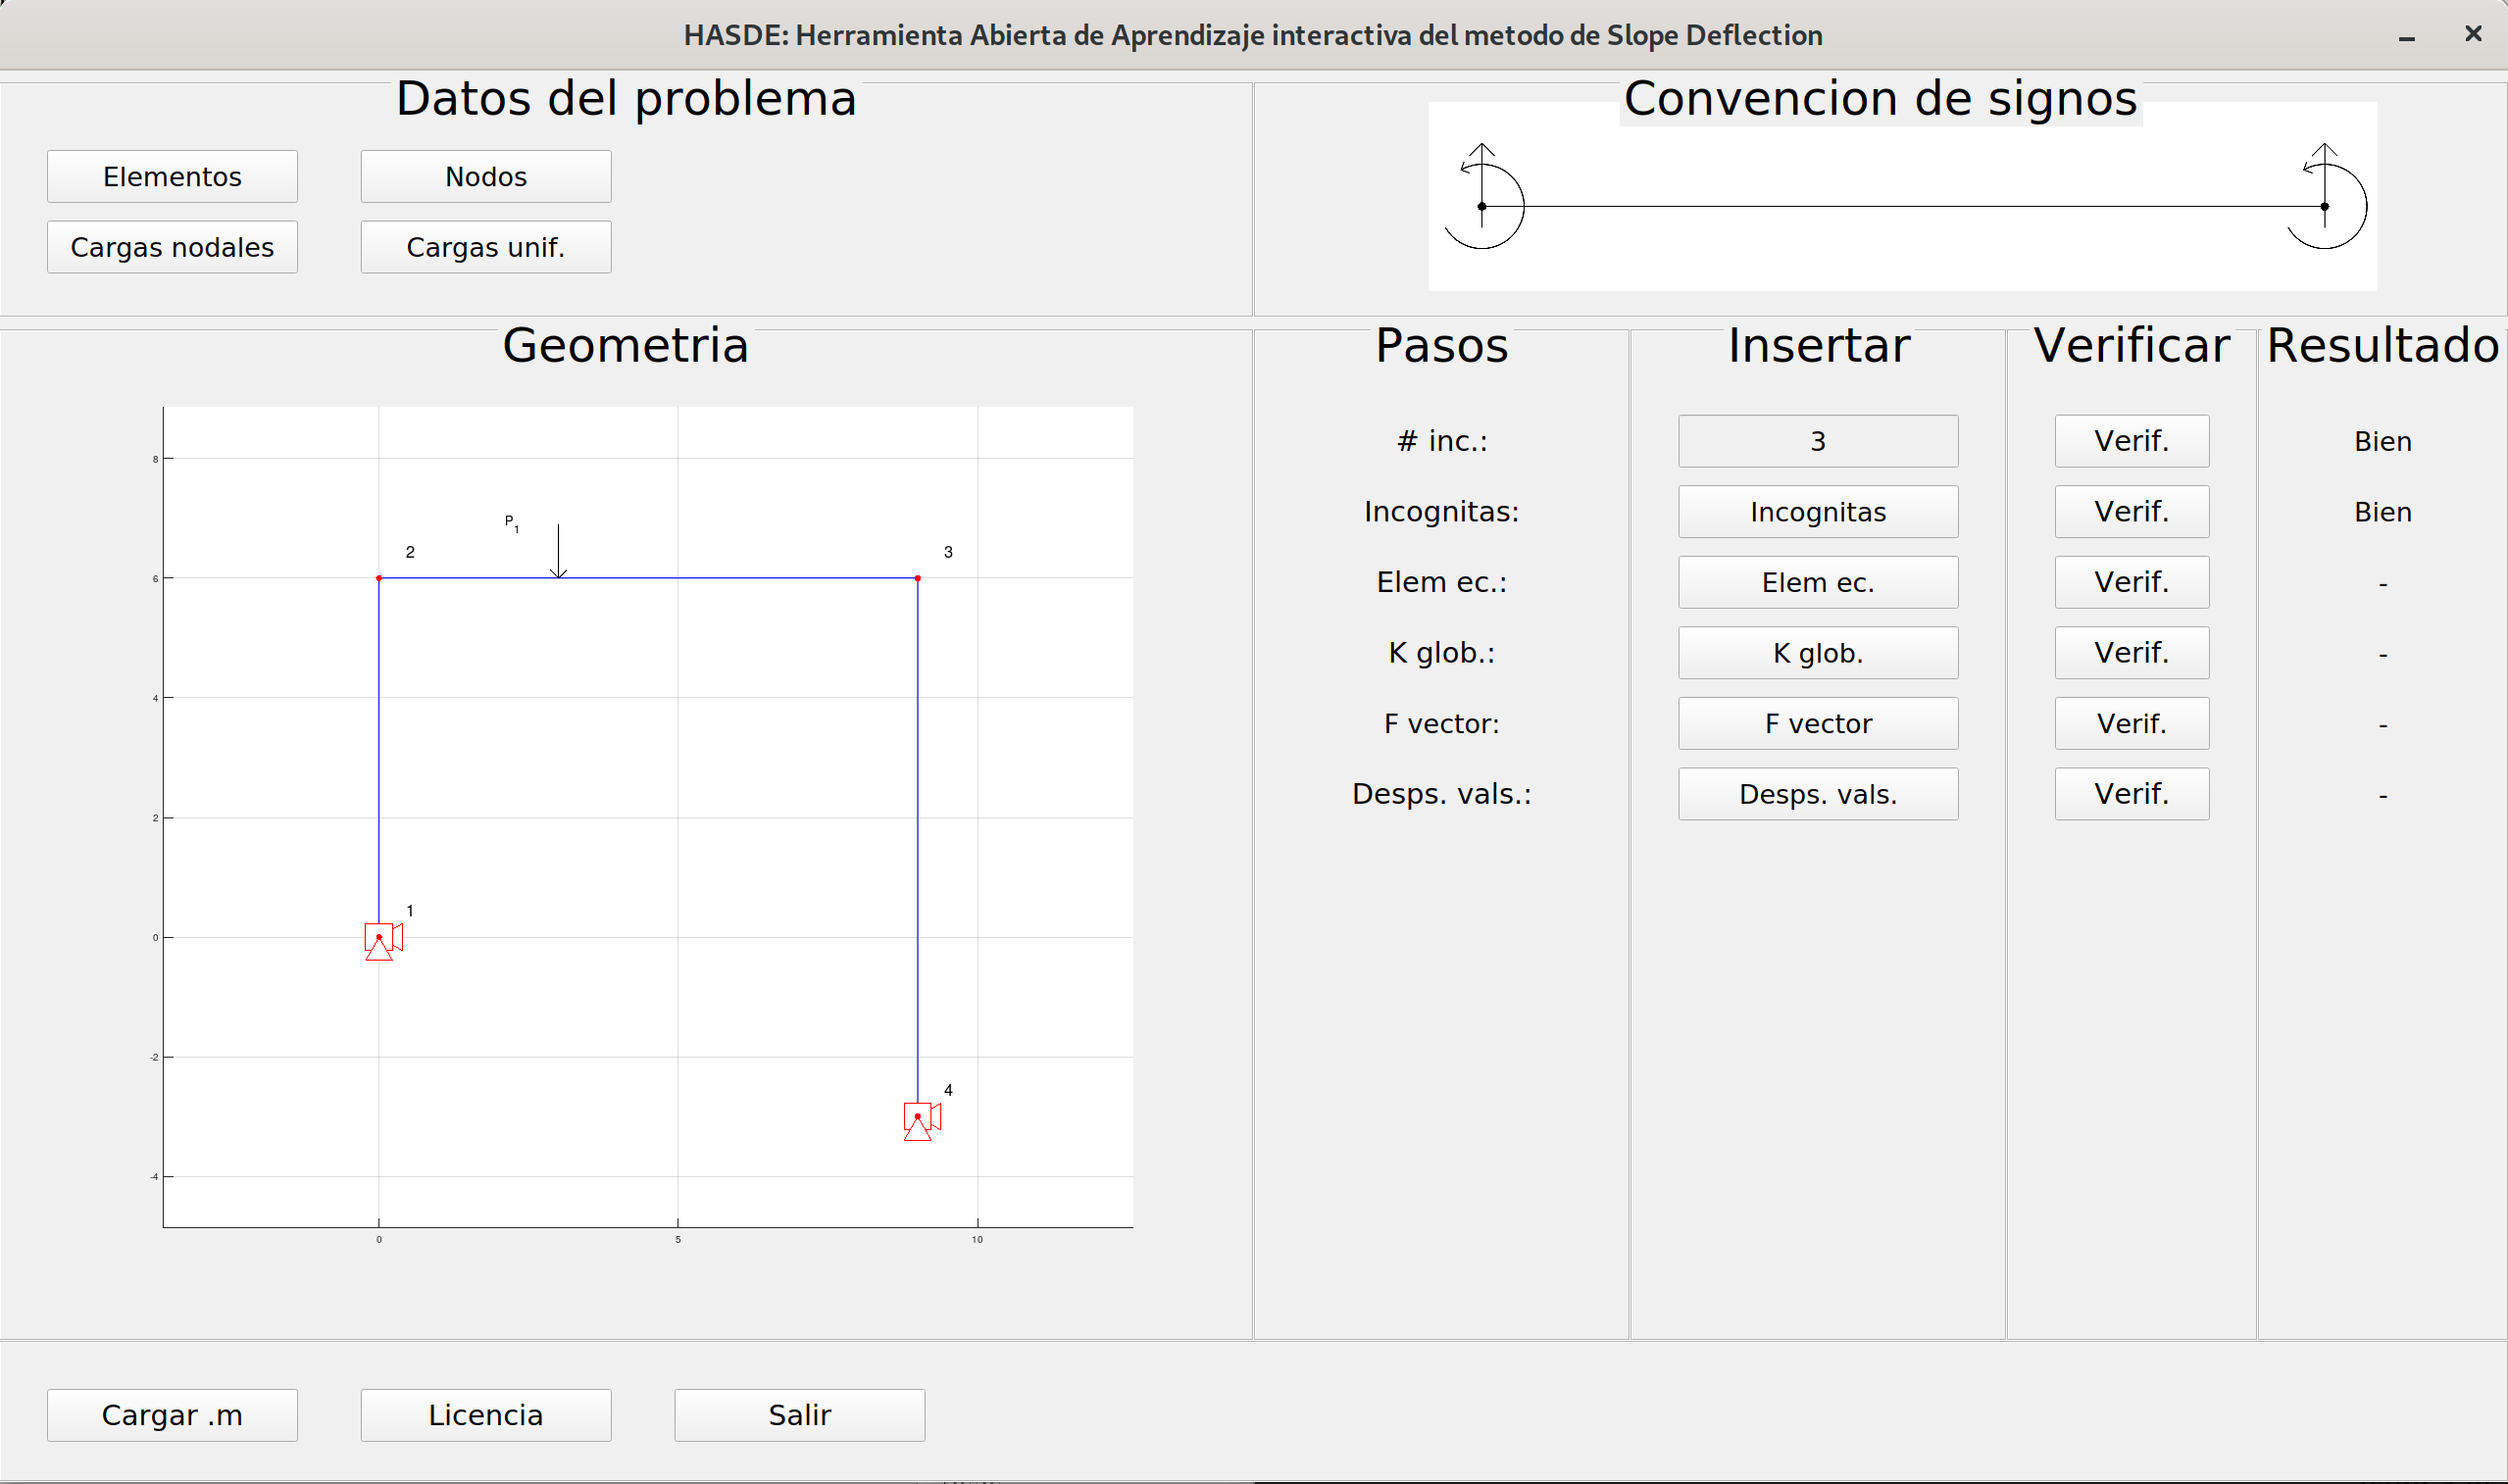
\includegraphics[width=\textwidth]{hasdeValid4}
	\end{center}
	\caption{Uso de HASDE en ejemplo.}
	\label{fig:eje}
\end{figure}

\paragraph{Ecuaciones de elemento}
El usuario puede ingresar las ecuaciones que desee y verificarlas con HASDE. Se debe indicar V o M en la primer columna para cortantes o momentos respectivamente.

\paragraph{Ecuaciones de elemento}
Este es el término independiente del sistema de ecuaciones acoplado para la obtención de los desplazamientos.

\paragraph{Matriz de rigidez global}
Esta es la matriz del sistema de ecuaciones acoplado para la obtención de los desplazamientos.

\paragraph{Valores de desplazamiento}
Los desplazamientos solución del problema.